\documentclass[10pt,a4paper]{article}
\usepackage[utf8]{inputenc}
\usepackage[T1]{fontenc}
\usepackage{amsmath}
\usepackage{amsfonts}
\usepackage{amssymb}
\usepackage{makeidx}
\usepackage{graphicx}
\usepackage{mdframed}
\usepackage{xcolor}
\usepackage{pgfplots}
\pgfplotsset{width=3in,compat=1.9}
\usepackage[left=1.00in, right=1.00in, top=1.00in, bottom=1.00in]{geometry}
\author{Tommaso Severini}
\title{Matematica - Fasci di rette}
\begin{document}
	
	%% mdframed definizione
\mdfdefinestyle{theoremstyle}{%
	linecolor=orange,linewidth=2pt,%
	frametitlerule=true,%
	frametitlebackgroundcolor=gray!20,
	innertopmargin=\topskip,
}
\mdtheorem[style=theoremstyle]{definition}{Definition}
	
	\maketitle
	
	Sappiamo come descrivere una retta conoscendo il suo coefficiente angolare ed un punto per cui questa retta passa attraverso la formula:
	\begin{equation*}
			y - y_0 = m(x - x_0)
	\end{equation*} 
	Se supponiamo che m possa variare e assumere qualsiasi valore appartenente a $\mathbb{R}$, essa diventerà l'equazione che descrive tutte le rette passanti per il punto $P(x_0; y_0)$. Questo insieme prende il nome di \textbf{fascio di rette proprio} si centro P.m L'unica retta non descritta da questa equazione è la retta $x = x_0$, in quanto il coefficiente angolare di questa retta tende a infinito.
	
	\begin{definition}[Fascio proprio di rette]
		L'equazione 
		\begin{equation*}
				y - y_0 = m(x - x_0)
		\end{equation*}
	dove $m$ è un elemento dei numeri reali, definisce il fascio di rette proprio di centro $P(x_0; y_0)$, esclusa l'equazione $x = x_0$
	\end{definition}

\begin{center}
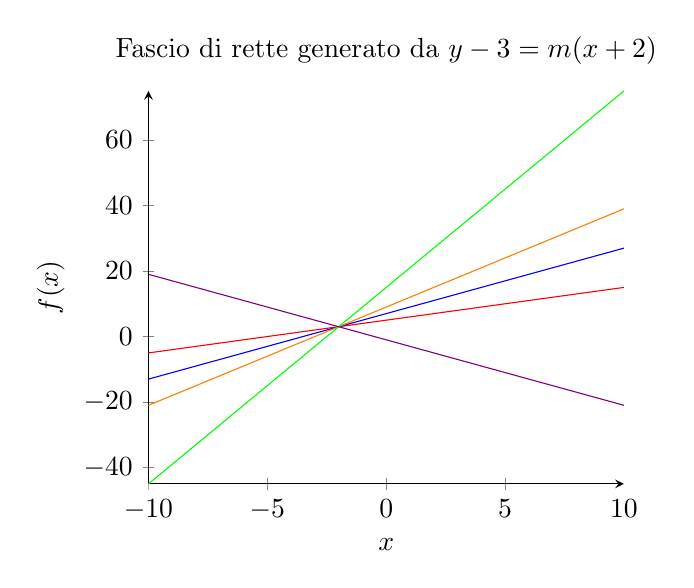
\begin{tikzpicture}[right]
	\begin{axis}[
		title={Fascio di rette generato da $y-3=m(x+2)$},
		axis lines = left,
		xlabel = $x$,
		ylabel = {$f(x)$},
		]
		%Below the red line is defined
		\addplot [
		domain=-10:10, 
		samples=100, 
		color=red,
		]
		{x + 5};
		%Here the blue line is defined
		\addplot [
		domain=-10:10, 
		samples=100, 
		color=blue,
		]
		{2*x + 7};
		
		\addplot [
		domain=-10:10, 
		samples=100, 
		color=orange,
		]
		{3*x + 9};
		
		\addplot [
		domain=-10:10, 
		samples=100, 
		color=green,
		]
		{6*x + 15};
		
		\addplot [
		domain=-10:10, 
		samples=100, 
		color=violet,
		]
		{-2*x - 1};
		
	\end{axis}
\end{tikzpicture}
\end{center}

	Consideriamo adesso l'insieme delle rette aventi lo stesso coefficiente angolare ma diversa intercetta con l'asse y. Esso avrà equazione:
	\begin{equation*}
		y = mx + k		\qquad	k \in \mathbb{R}
	\end{equation*}
	Questo insieme prende il nome di \textbf{fascio di rette improprio}. Nel caso di rette verticali, l'equazione del fascio diviene $x = k$.
	
	\begin{definition}[Fascio di rette improprio]
	L'equazione 
		\begin{equation*}
			y = mx + k \qquad k \in \mathbb{R}
		\end{equation*}
	definisce un fascio di rette di rette improprio. Esso sarà composto da  rette parallele di coefficiente angolare $m$. 
	
	
	\end{definition}

\begin{center}
	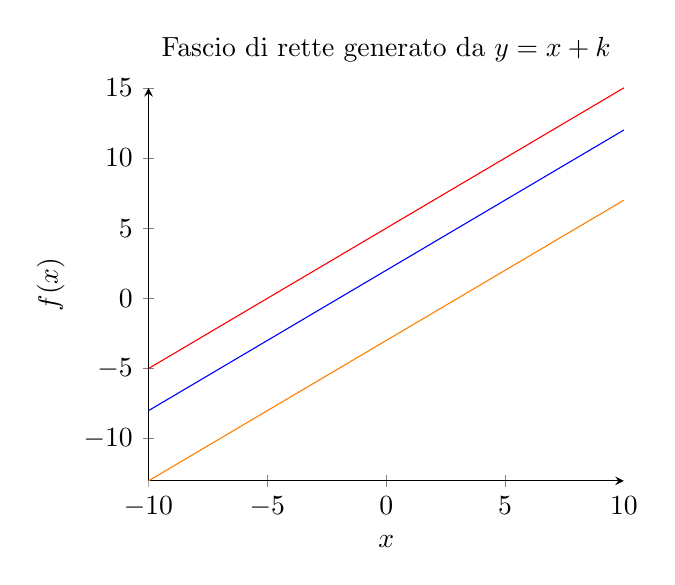
\begin{tikzpicture}
		\begin{axis}[
		title={Fascio di rette generato da $y = x + k$},
		axis lines = left,
		xlabel = $x$,
		ylabel = {$f(x)$},
		]
		%Below the red line is defined
		\addplot [
		domain=-10:10, 
		samples=100, 
		color=red,
		]
		{x + 5};
		\addplot [
		domain=-10:10, 
		samples=100, 
		color=blue,
		]
		{x + 2};
		\addplot [
		domain=-10:10, 
		samples=100, 
		color=orange,
		]
		{x - 3};
		\end{axis}
	\end{tikzpicture}
\end{center} 

Bisogna anche ricordare che un fascio di rette proprio può essere generato da due rette date $r$ e $s$:
	\begin{definition}[Fascio generato da due rette]
		Date due rette $r$ e $s$, il fascio generato da queste rette sarà dato dall'equazione 
		\begin{equation*}
			ax + by + c + k(a'x + b'y + c')= 0	\qquad	k \in \mathbb{R}
		\end{equation*}
		Dove $ax + by + c$ e $a'x + b'y + c'$ rappresentano le rette $r$ e $s$.
	\end{definition}
	
\end{document}